%%%%%%%%%%%%%%%%%%%%%%%%%%%%%%%%%%%%%%%%%%%%%%%%%%%%%%%%%%%%%%%%%%%%%%%%%%%%%%%
%% Active Learning Machine Learning Methodology
%%
%%
%% Points to mention:
%%    Voronoi is used because it is insensitive to volume expansions of structure
%%    TODO: Explain PCA analysis
%%    TODO: Get PCA reference
%%
%% TODO:
%%    Why AB2 and AB3
%%    TEMP
%%%%%%%%%%%%%%%%%%%%%%%%%%%%%%%%%%%%%%%%%%%%%%%%%%%%%%%%%%%%%%%%%%%%%%%%%%%%%%%


% ################################# Paragraph #################################
% %%%%%%%%%%%%%%%%%%%%%%%%%%%%%%%%%%%%%%%%%%%%%%%%%%%%%%%%%%%%%%%%%%%%%%%%%%%%%
% General intro to AL scheme
% Basic gist, i.e. define our candidate space of materials to explore within
% (we do this by looking taking all structurally unique systems in DBs)
% To start the AL we take the few systems that have DFT calcs (more generally
% we can just choose random structures)
% We then build a surrogate model (GP, initially really bad) to predict the
% stability of the entire candidate space
% %%%%%%%%%%%%%%%%%%%%%%%%%%%%%%%%%%%%%%%%%%%%%%%%%%%%%%%%%%%%%%%%%%%%%%%%%%%%%
% | - Paragraph start
Our machine learning accelerated materials discovery method proceeds through the following steps
%
First, the dataset of candidate materials is constructed.
%
This data set will define the totality of materials that will be considered by the search algorithm,
this is done because the search space of materials is not a continous space but a discrite array of individual structures.
%
Next, the dataset of materials is transformed into a vectorial representation by using a fingerprinting method that encodes the relevent chemical and structural information.
%

% __|


% ################################# Paragraph #################################
% %%%%%%%%%%%%%%%%%%%%%%%%%%%%%%%%%%%%%%%%%%%%%%%%%%%%%%%%%%%%%%%%%%%%%%%%%%%%%
% Data prep. | Unique Structures | Atom subst., V relax | Fingerprinting
% %%%%%%%%%%%%%%%%%%%%%%%%%%%%%%%%%%%%%%%%%%%%%%%%%%%%%%%%%%%%%%%%%%%%%%%%%%%%%
% | - Paragraph start
The structures that comprise the candidate data set were constructed by parsing for structurally unique systems in the OQMD and Materials Project DFT databases.
%
The structural uniqueness was performed using a space-group symmetry classification scheme developed by Jain et al. \cite{Jain2018},
which can classify a structure based on its composition and structure.
 (see SI for more details on the structural classification scheme).
%
This structural classification scheme can directly serve as a structural fingerprint and has successfully been applied towards the prediction of formation energies of inorganic compounds \cite{Jain2018}
%
To focus the scope of the study, only AB2 and AB3 stoichiometries were parsed from the databases.
%
The AB2 formula was chosen because it includes \rIrOtwo, the known most stable polymorph of IrO2.
%
Importantly, AB3 was chosen to include high valency IrO3 structures in our search.
%
The results of the classification scheme resulted in a XYZ AB2 and XYZ AB3 structural prototypes for which iridium and oxygen were replaced for A and B sites, respectively.
%
Finally, a coarse isotropic volume relaxation based on atomic radii was performed on the structures to accommodate the atomic radii of iridium and oxygen into the lattice.
%
Finally, a Voronoi tessellation based fingerprinting scheme developed by Ward et al. \cite{Ward2017} was used to encode the relevant chemical information for each structure into a vector quantity of length 271.
%
The Voronoi based method was used because it is insensitive to volume relaxation.
%
Separate, indpedent models were used for IrO2 and IrO3 to reduce the complexity of the space, this has the addtional effect of making a large number of the fingerprint descriptors reduendant.
% How many columns of the 271 are redundant if stoich and composition are frozen
As a result, the 271 length feature space is reduced to a TEMP length vector.
%
PCA was used to reduce the dimensionality of the feature space from 271 to 20 features such that 99 \% of the variance is captured \cite{Tipping1999}.
% __|


% ################################# Paragraph #################################
% %%%%%%%%%%%%%%%%%%%%%%%%%%%%%%%%%%%%%%%%%%%%%%%%%%%%%%%%%%%%%%%%%%%%%%%%%%%%%
% Iterative Training of Gaussian Process
% TODO go through fingerprinting here, not previous part
% %%%%%%%%%%%%%%%%%%%%%%%%%%%%%%%%%%%%%%%%%%%%%%%%%%%%%%%%%%%%%%%%%%%%%%%%%%%%%
% | - Paragraph start
The active learning algorithm proceeds through iterative ML training, prediction, and acquisition steps and is visualized in figure TEMP.
%
Although we could use practically any regression technique, we employed the Gaussian process (GP) regression model because it offers a high degree of flexibility and, most importantly, built-in error quantification.
% TODO: Does the aquisition function we use have a name?
Error quantification on the predicted formation energies is important because its used in the aquisition criteria.
%
Further details on the GP model, including hyper parameter information, is including in the SI.
%
The aquisition is made by selecting the $N$ systems with the lowest value of the aquisition function.
%
The aquistion function is defined as the predicted formation energy minus the uncertainty,
% TODO: Write aquisition function here, again does it have a name
$a = b + c$
%
The value of $N$ determines how many structures are selected for DFT calculations,
and as such, determines the degree of parallization of the routine.
%
Small values of N result in an algorithm that is slow, as every DFT calculation is performed serially.
% TODO: Is this statement true?
Larger values of N speed up the algorith, but potentially decreases the efficiency of the algorithm by TEMP TEMP.
%
Here we chose a value $N=10$.
%
The aquired strcutres are initially volume relaxed, followed by a full relaxation of all of the atomic coordinates,
see SI for additional details on the DFT methodology.
% This is wordy
The AL loop proceeds until convergence is achieved, which here is defined as the point at which the model has determined the lowest $N$ structures and has acheived a degree of accuracy for the candidate space such that no structures have formation energies with a lower uncertainty bound lower than the most stable $N$ structures.

% __|


\begin{enumerate}
  \item Candidate space of structures is generated
  \item Initial seed data is used to train a ML model
  \item ML model predicts energy of entire candidate space
  \item Most valuable calculation(s) is selected using acquisition function
  \item DFT calculation(s) is(are) performed to obtain additional training data points
  \item ML model is retrained with additional data
  \item Repeat steps (TEMP) through (TEMP) until convergence criteria is reached
  % \item TEMP
\end{enumerate}

% | - Figure | Active Learning Algorithm **************************************
\begin{figure*}
\centering
\makebox[\textwidth][c]{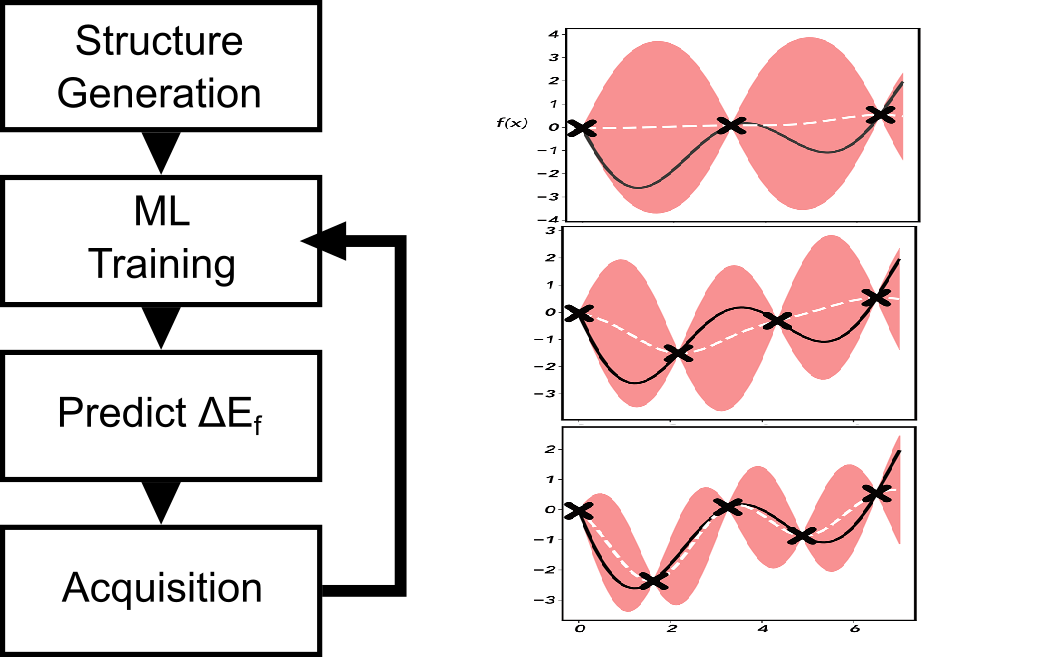
\includegraphics
  {02_figures/Surrogate_model_mine.png}
  }
\caption{\label{fig:all_diagram}
(a) Active learning algorithm diagram.
First the candidate space of structures is generated,
next, the machine learning model is trained on any available DFT formation energy data.
The trained ML model is then used to predict the DE of the entire candidate space.
Finally, an acquisition step is performed to pick the next most valuable calculation to perform an-initio DFT on
% -----------------------------------------------------------------------------
(b) Toy model demonstrating a GP model converging with each subsequent iteration.
% -----------------------------------------------------------------------------
}
\end{figure*}
% __|




% #############################################################################
% | - __old__
% ################################# Paragraph #################################
% AB2 Structures Ankit
% - There are XYZ unique AB2 structures (or multiples, e.g. A2B4)
% - Of those we found 697 unique AB2 prototypes (unique SG/Wyckoff combination) in OQMD/MP
% - To generate our test set we substituted Ir for A and O for B, then isotropically expanded cell volume to constrain a minimum Ir-O distance of XYZ
% - Next translated each of the 697 structures to be described by 271 features (invariant to isotropic expansion/compression), then reduced to 30 using PCA, described in methods XYZ
% - To generate initial training data use existing DFT. Not enough on \ce{IrO_2}, so used OQMD to generate initial training data from nearest structures in phase space, described in Methods XYZ. Training set of 30 structures in SI XYZ.
% __|
